\section{Atlassian:团队合作的力量}

\textbf{Atlassian为全球领先的项目管理、内容协同SaaS厂商}。Atlassian位于澳大利亚,提供面向企业业务流程的协同办公产品,多年位居Gartner魔力象限的领导者象限。Atlassian主要面向软件开发者,也向企业技术人员、知识工作者等群体扩展。财富500强中的大多数以及全球超过240,000家各种规模的公司都依赖Atlassian的解决方案来帮助他们的团队更好地合作并按时交付高质量的结果。在,包括Jira软件、Confluence、Jira服务管理、Trello、BitBucket和Jira Align等。
\begin{figure}[H]
    \centering
    \begin{minipage}{0.38\linewidth}
        \caption{Atlassian位于魔力象限的领导者}
        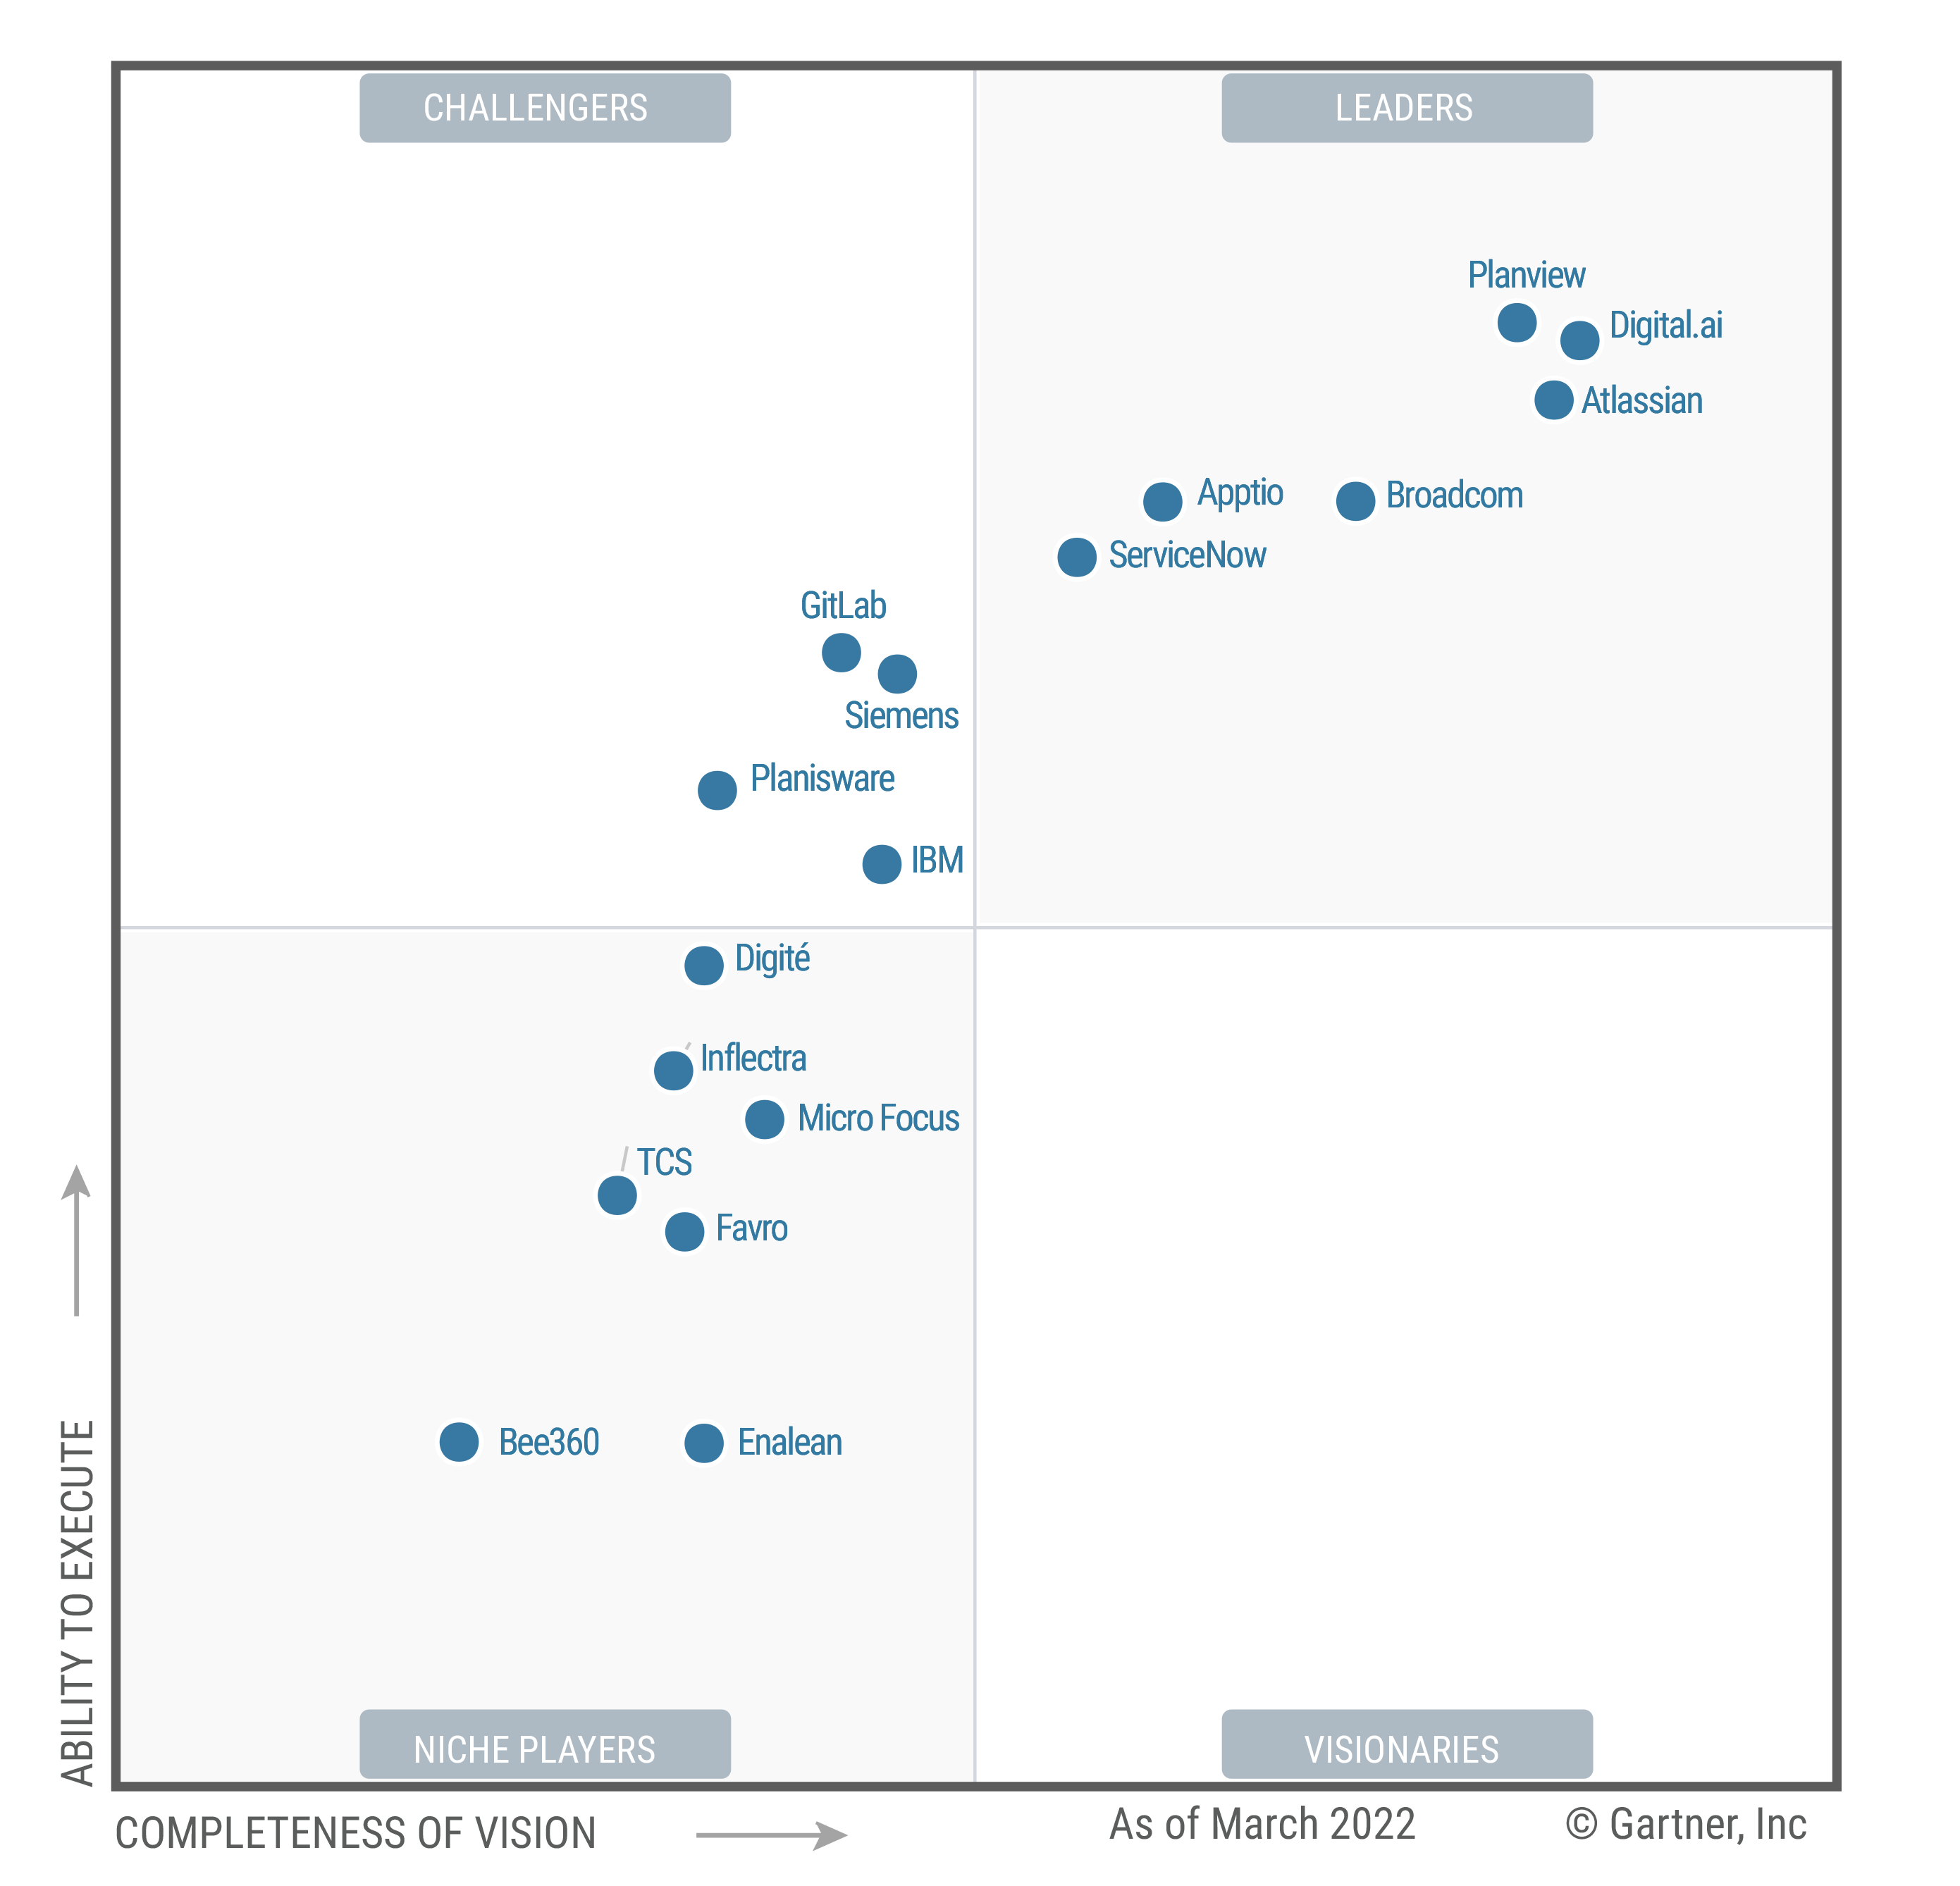
\includegraphics[width=\linewidth]{img/gartner.png}
        \footnotesize{资料来源:Gartner}
    \end{minipage}
    \begin{minipage}{0.58\linewidth}
        \caption{Atlassian用户数}
        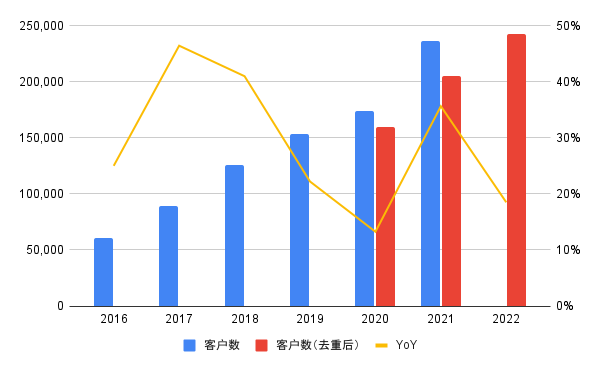
\includegraphics[width=\linewidth]{img/customers.png}
        \footnotesize{资料来源:公司公告。注:1Q22更换统计口径,不同产品的用户数去重}
    \end{minipage}
\end{figure}

\textbf{Jira和Confluence是Atlassian的核心产品,满足软件开发行业敏捷开发等需求}。Atlassian公司成立于2002年,在成立两年内发布了拳头产品Jira和Confluence,并在2010年将产品迭代上云,于2015年上市。Atlassian还通过不断并购扩大产品矩阵,如项目管理软件Trello、代码托管网站Bitbucket、Git客户端SourceTree等。这些软件都与Jira和Confluence高度集成,形成丰富的产品生态。
\begin{figure}[H]
    \caption{Atlassian公司历史}
    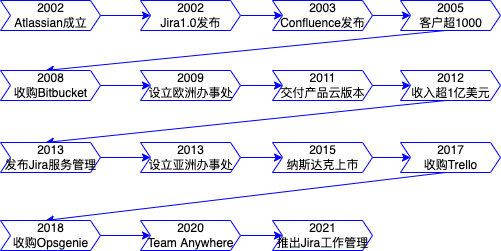
\includegraphics[width=\linewidth]{img/timeline.drawio.png}
    \footnotesize{资料来源:公司公告}
\end{figure}

\subsection{Atlassian的财务水平}

\textbf{Atlassian 的收入主要来自订阅收入、永久许可、维修收入和其他来源}。其中:
\begin{enumerate}
    \item 订阅是 Atlassian 收入的主要来源,占比逐年提高,1Q23占总收入的 80\%。订阅收入主要由活跃许可证的数量和大小、产品类型和许可证的价格驱动,预计未来受益于云计算进一步普及仍将持续增加。
    \item 永久许可证收入包括从向新客户销售许可证、增加现有客户中的用户数量和向现有客户增加许可证中确认的收入。2022年Atlassian取消了永久许可证业务,鼓励用户转向云订阅。
    \item 维护收入是指为永久许可产品向客户支持所获得的费用,但受永久许可证不再签发影响有所萎缩。
    \item 其他收入包括在 Atlassian Marketplace销售第三方应用程序和培训服务的费用。Atlassian Marketplace类似App Store,在第三方销售收入中抽成比例为15-25\%。这部分收入随Atlassian生态的逐步完善吸引更多第三方应用开发者,增长也非常迅速,但体量较小。
\end{enumerate}
\begin{figure}[H]
    \caption{Atlassian分业务收入(万美元)}
    \begin{center}
        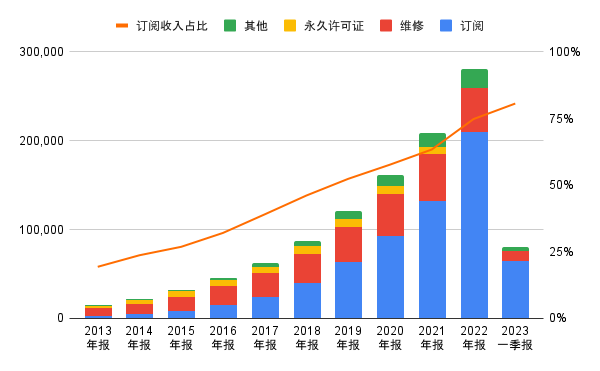
\includegraphics[width=\linewidth]{img/revenue.png}
    \end{center}
    \footnotesize{资料来源:同花顺iFind}
\end{figure}

\textbf{费用上,Atlassian轻营销、重研发}。一般的SaaS和软件厂商由于大量的营销费用呈现出高毛利、低净利的情况。Atlassian采用直销的方式降低营销成本,并且拳头产品的口碑非常好,一度不需要销售人员。Atlassian 销售费用率始终低于研发费用率,销售费用率常年在 20\%上下浮动(正常的 SAAS 企业销售费用率在40\%-60\%,个别企业甚至在 80\%左右)。此外Atlassian重研发,不断研发新功能以贴合软件行业的快速发展。近期Atlassian出于逆周期扩张的战略S\&M、G\&A费用率均有所增加。
\begin{figure}[H]
    \caption{Atlassian费用水平(万美元)}
    \begin{center}
        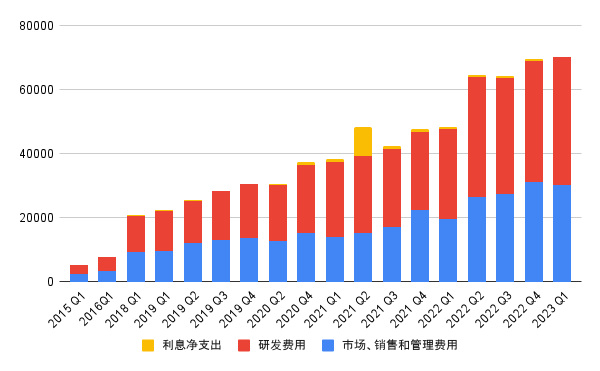
\includegraphics[width=0.8\linewidth]{img/cost.png}
    \end{center}
    \footnotesize{资料来源:同花顺iFind}
\end{figure}

\textbf{Atlassian保持长期盈利,non-GAAP净利持续为正}。Atlassian在未上市时便保持了长期的盈利,上市后营业利润率保持增长趋势,但在2022年出于公司战略营业利润率有所下滑。
\begin{figure}[H]
    \caption{non-GAAP口径下Atlassian财务状况}
    \begin{center}
        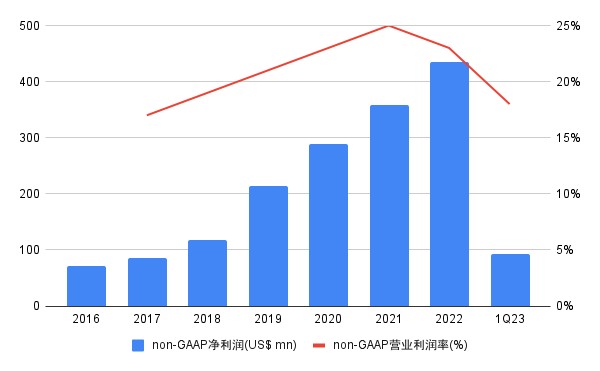
\includegraphics[width=0.7\linewidth]{img/non-GAAP.png}
    \end{center}
    \footnotesize{资料来源:公司公告}
\end{figure}

\subsection{Atlassian的产品线}
Atlassian的产品线主要有以下四条:用于团队计划和项目管理的 Jira系列等、用于团队内容创建和协作的 Confluence和Trello等、用于团队编写代码和管理审查的 Bitbucket和SourceTree等、以及用于身份与安全的Atlassian Access等。

\textbf{Jira在敏捷开发时代为组织提供了工作流}。Jira 是一个复杂而灵活的工作流管理系统,帮助团队计划组织、跟踪Bug和管理项目。Jira Software 专为软件团队中的每位成员构建,可供其用于规划、跟踪和发布卓越的软件,具有规划、跟踪、发布、报告和自动化五大用途。Jira Service连接开发、IT 运营和业务团队,快速响应需求变更,提升开发敏捷度。Atlassian旗下的另一款软件Opsgene则集中管理警报,在业务逻辑发生问题时及时通知给正确的人。此外Jira也集成到Atlassian体系外的常用办公软件,如Slack等。
\begin{table}[H]
    \caption{Jira Software 五大用途}
    \begin{tabular}{ll}
        \toprule
        用途  & 内容                             \\
        \midrule
        规划  & 通过用户故事、事务和任务,将宏大计划分解为易于管理的部分   \\
        跟踪  & 追踪bug与需求,排定整个环境中团队工作的优先次序并进行讨论 \\
        发布  & 加速交付,同时保证自己所拥有的信息保持最新          \\
        报告  & 根据直观的实时数据,在整体环境下提升团队绩效         \\
        自动化 & 通过无代码自动化功能,节省时间、保持专注、顺畅工作流     \\
        \bottomrule
    \end{tabular}
    \footnotesize{资料来源:Atlassian}
\end{table}

\textbf{Confluence作为企业内部的知识wiki,实现企业内部的知识共享}。Confluence 是一个社会性的、灵活的内容协作平台,用于创建、共享、组织和讨论项目。不同于一般的协作文档,Confluence针对技术团队提供了大量的规范模版,并支持富媒体编辑,满足技术文档中的UML类图、Visio图、流程图的需求;文档中还可以内嵌评审流程,不止于仅仅@某人,关联研发过程。通过软件开发者中的盛誉,Confluence也向企业技术人员、知识工作者等群体破圈传播。
\begin{figure}[H]
    \caption{Confluence可以与Jira集成}
    \begin{center}
        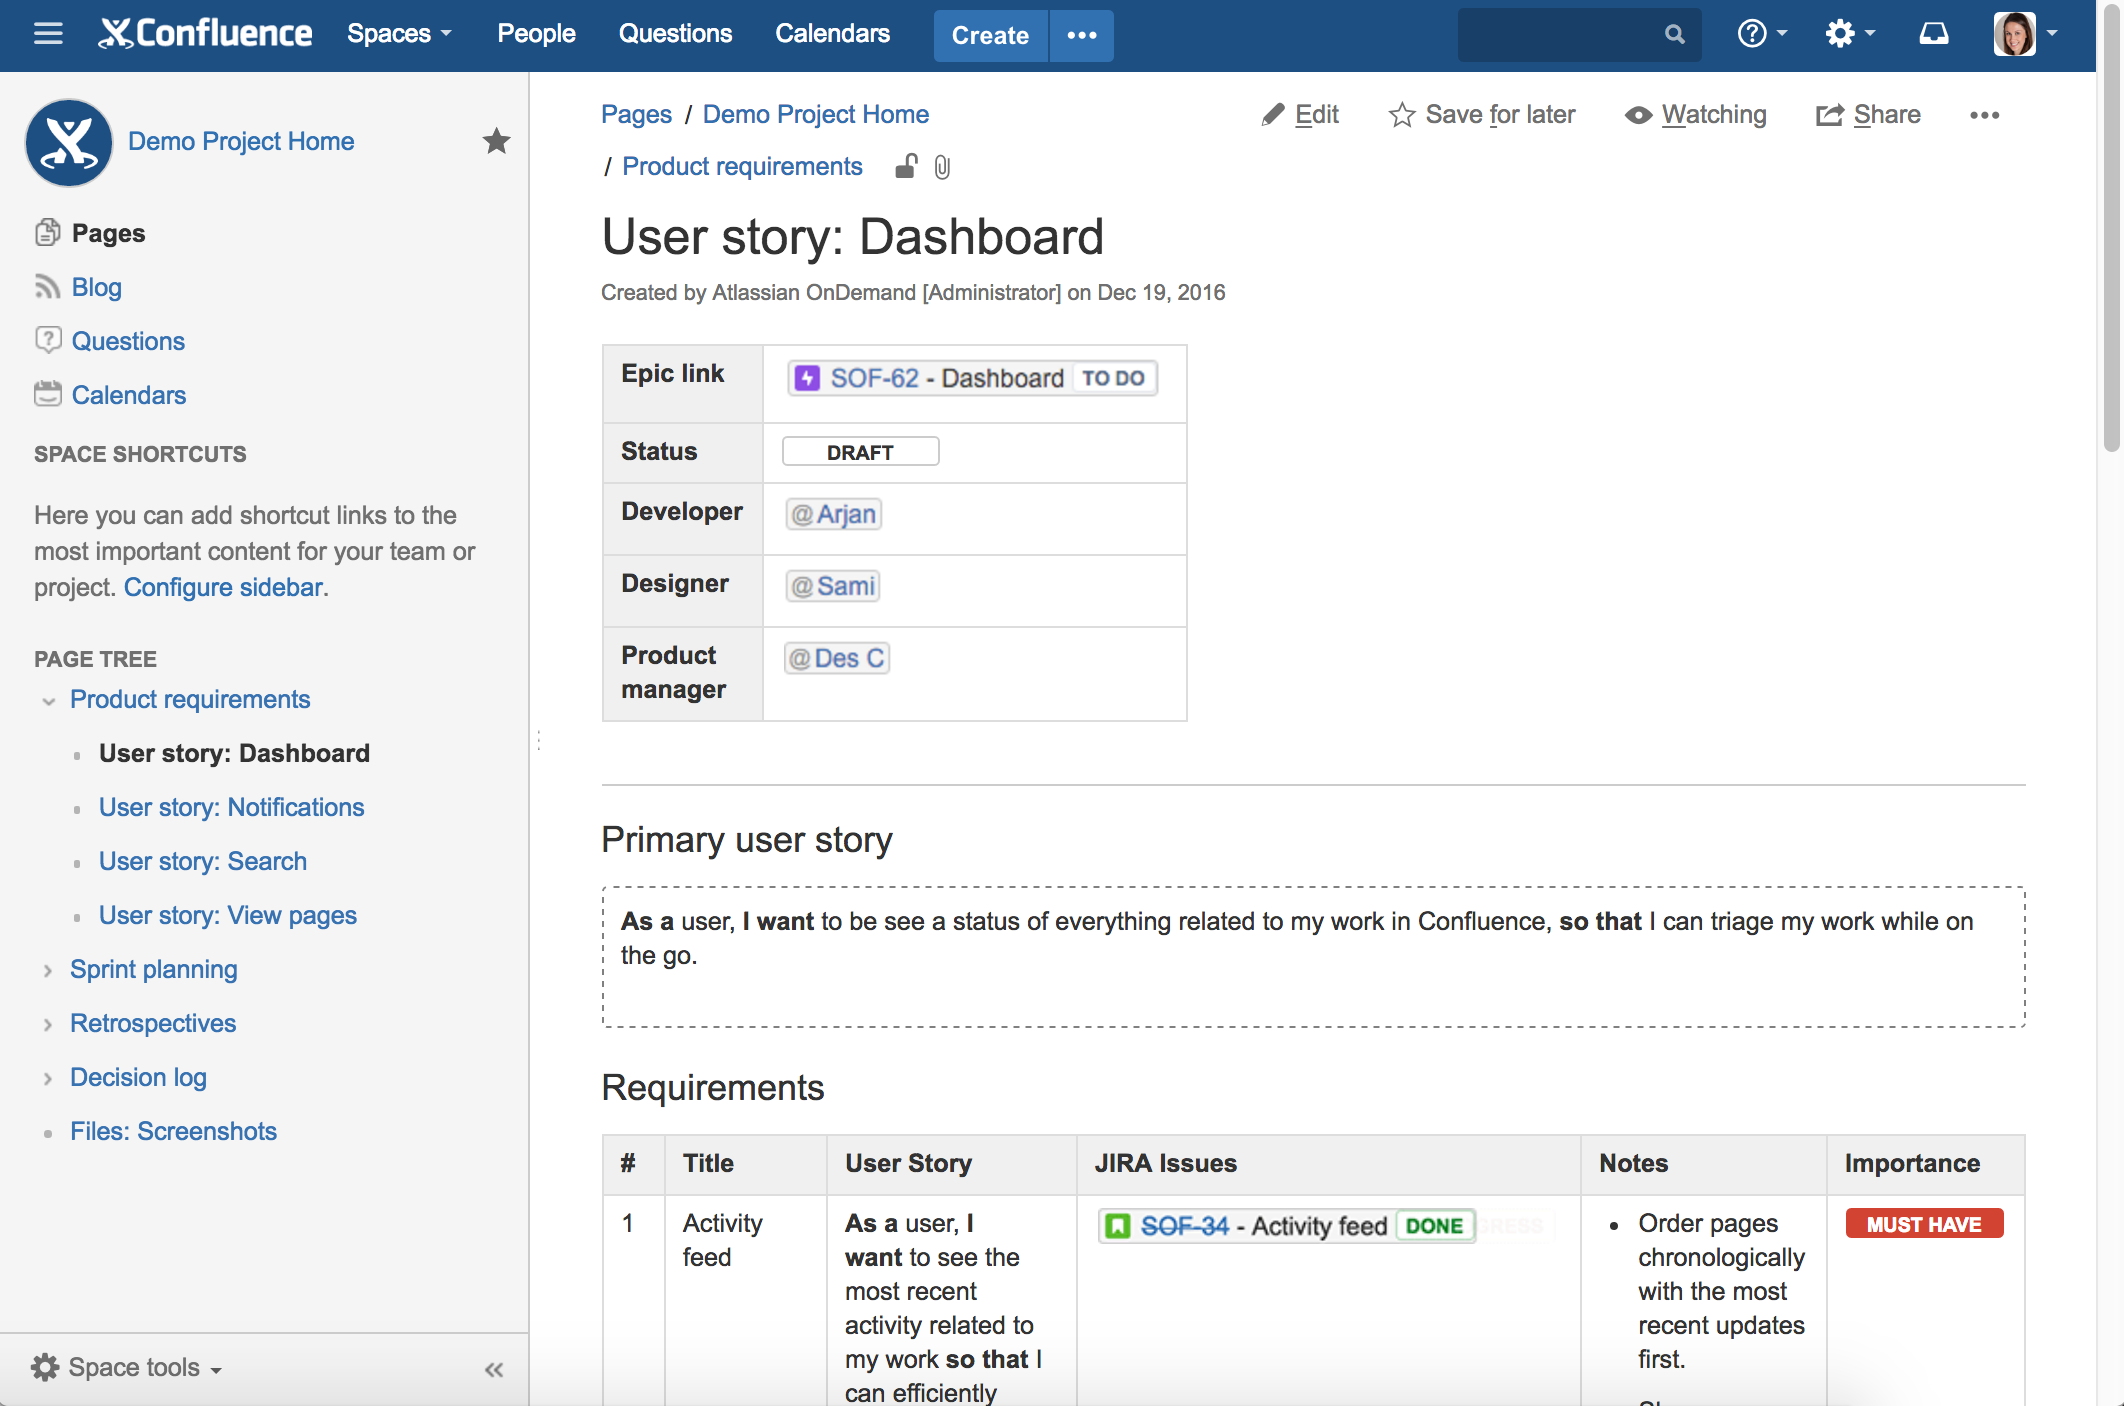
\includegraphics[width=0.8\linewidth]{img/Using+Confluence+with+JIRA.png}
    \end{center}
    \footnotesize{资料来源:Atlassian Documentation}
\end{figure}

\textbf{Trello专注于更通用的任务管理}。Jira所包含的任务管理主要是和敏捷开发相关的,以开发一个软件产品为目标。Trello则提供了更通用的看板,提供了任务进度等要素,帮助团队对任务进行计划。
\begin{figure}[H]
    \begin{minipage}{0.48\linewidth}
        \caption{Jira任务管理基于产品目标}
        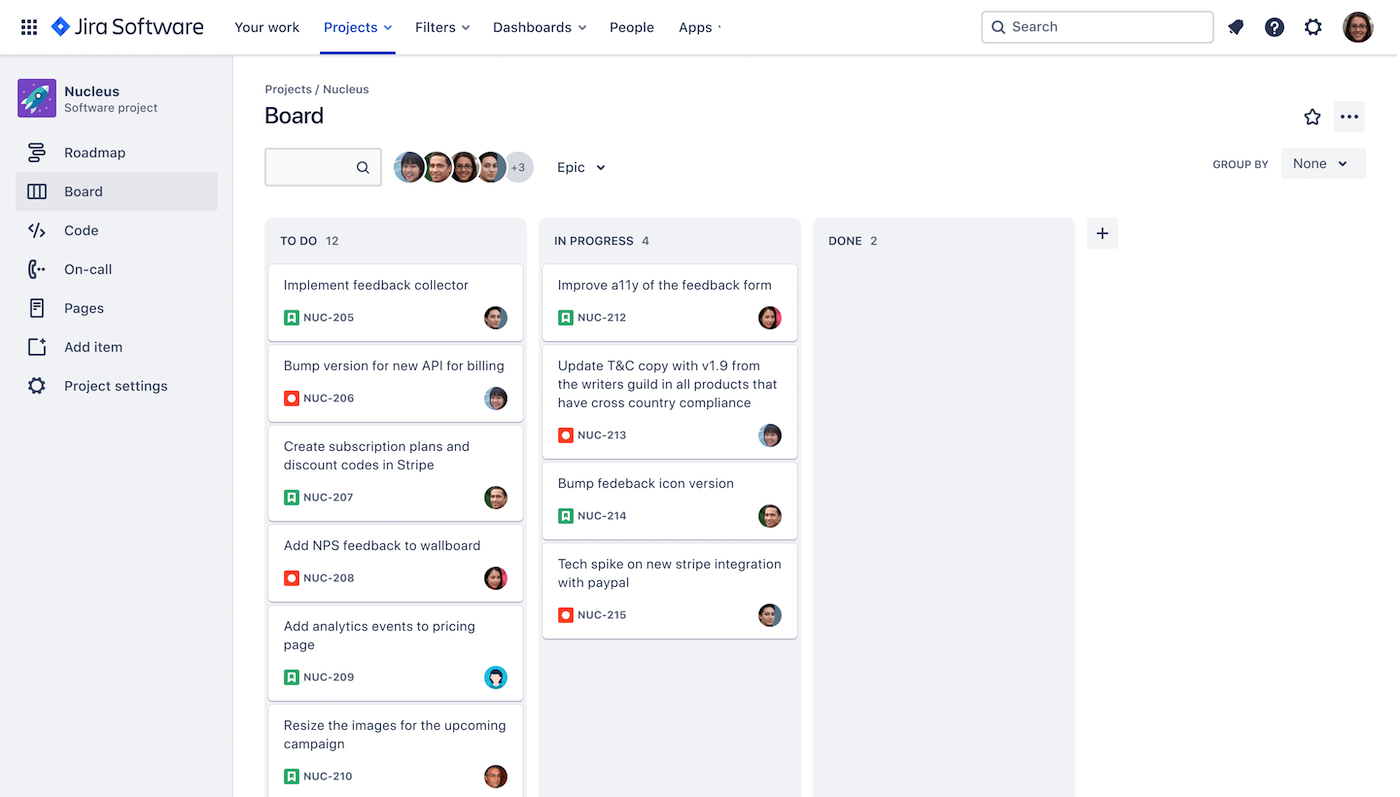
\includegraphics[width=\linewidth]{img/jira.png}
    \end{minipage}
    \begin{minipage}{0.48\linewidth}
        \caption{Trello任务管理更为通用}
        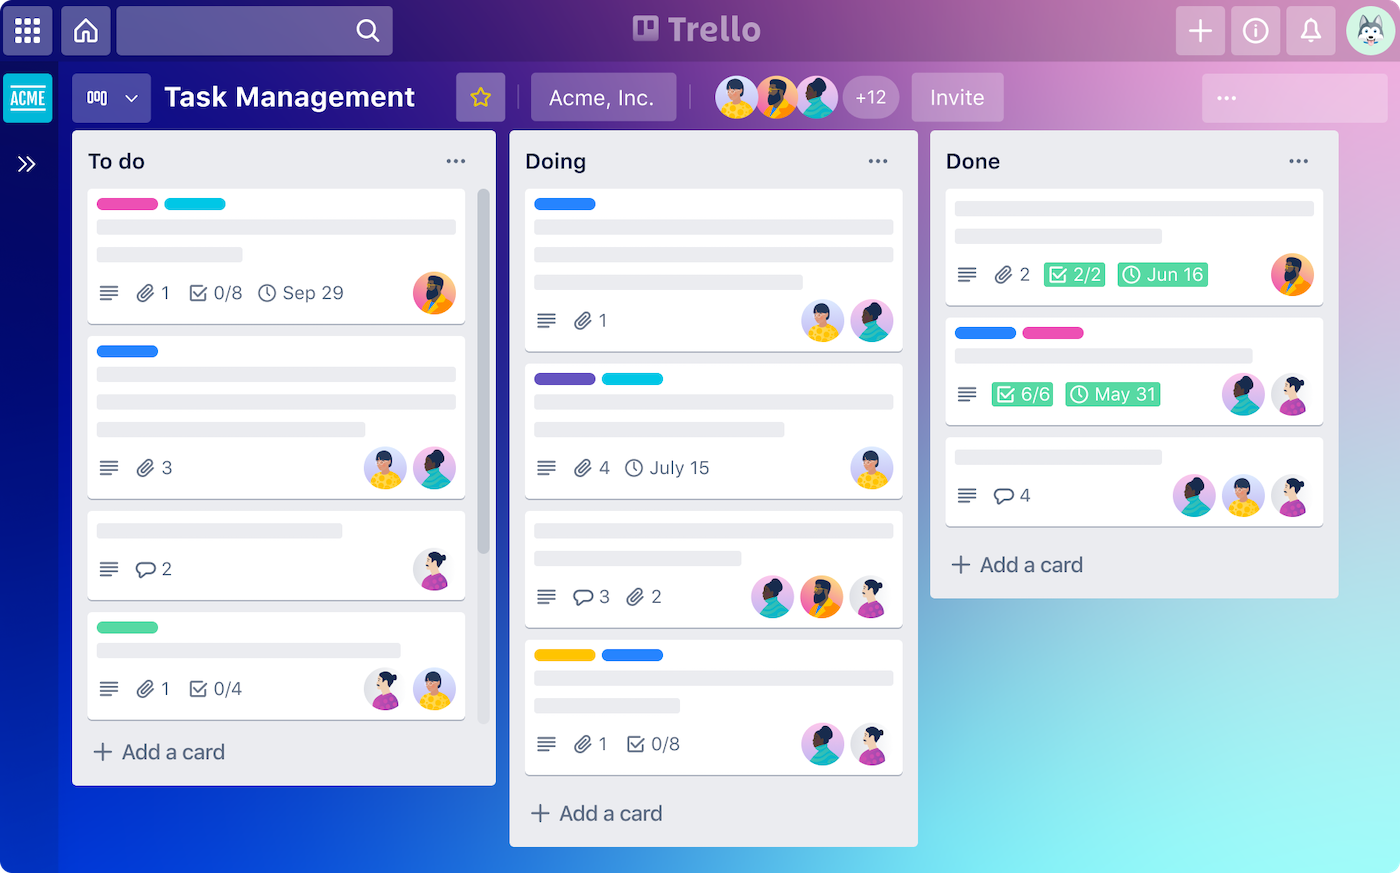
\includegraphics[width=\linewidth]{img/Trello.png}
    \end{minipage}
    \footnotesize{资料来源:technologyadvice}
\end{figure}

\textbf{Bitbucket类似GitHub与GitLab,对Jira有更强的集成}。BitBucket 是 2008 年创建的源代码托管网站,采用 Mercurial 和 Git 作为分布式版本控制系统,同时提供免费账户和商业计划。2010 年被 Atlassian 收购,与 Atlassian 的其他服务(Jira、SourceTree、Bamboo、Crucible等)高度集成,其主要市场是大型企业。

Atlassian Access等简化了 Okta 和 SSO 的登录流程,可将用户的 Atlassian 云产品与身份提供商连接起来。
